

\chapter{Procedures for system assembly/installation/testing/commisioning} \label{CHAPTERASSEMBLY}

\section{System assembly}
\subsection{Cable}
\subsubsection{Construction of ACT/E - Cable for motor encoder} \label{CONSTRUCTION:ACTE}

\subsubsection{Construction of ACT/H - Cable for motor Hall effect sensor} \label{CONSTRUCTION:ACTH}

\subsubsection{Construction of ACT/M - Cable for motor supply} \label{CONSTRUCTION:ACTM}

\subsubsection{Construction of CAN/D-D - Cable for CAN between drivers} \label{CONSTRUCTION:CANDD}

\subsubsection{Construction of CAN/I-Dc - Cable for CAN between driver and an interface (shield cut)} \label{CONSTRUCTION:CANIDc}

\subsubsection{Construction of CAN/I-Dp - Cable for CAN between driver and an interface (shield pass)} \label{CONSTRUCTION:CANIDp}

\subsubsection{Construction of CAN/I-I - Cable for CAN between interfaces} \label{CONSTRUCTION:CANII}

\subsubsection{Construction of CAN/I-PC - Cable for CAN between PC and an interface} \label{CONSTRUCTION:CANIPC}

\subsubsection{Construction of CAN/Out - Outdoor cable for CAN between modules} \label{CONSTRUCTION:CANOut}

\subsubsection{Construction of LAN/I-S - Cable for Ethernet between Ethernet Switch and an interface} \label{CONSTRUCTION:LANIS}

\subsubsection{Construction of LAN/Out - Outdoor cable for Ethernet between modules} \label{CONSTRUCTION:LANOut}

\subsubsection{Construction of LAN/S-D - Cable for Ethernet between Ethernet Switch and a device} \label{CONSTRUCTION:LANSD}

\subsubsection{Construction of USB/DAQ - Cable for USB between DAQ and PC} \label{CONSTRUCTION:USBDAQ}
\subsubsection{Crimping Molex Micro-Fit 3.0\texttrademark Family} \label{CRIMPINGmicro}
For connecting wires to a Molex Micro-Fit 3.0\texttrademark connector from 43025-xxxx family (sections~\ref{DEVICE:microCAN} and~\ref{DEVICE:microHall}), you first need to crimp the edge of these wires in the Molex crimp terminal from 43030-xxxx family (section~\ref{DEVICE:microCrimp}). For this, you should perform the following steps:
\begin{enumerate}
  \item Use the tool "Molex Hand Crimper Tool Part Number: 63819-0000" (see section~\ref{DEVICE:TOOLCRIMPERmicro}).
  \item For each wire to be connected, use a cutting plier (like the one described in section~\ref{DEVICE:TOOLPLIERCUTTING}), strip the wire envelop, leaving 2mm copper exposed.
  \item Place the wire and the crimp terminal according to figure~\ref{FIG:CRIMPmicro1}.
  \item Use the Molex Hand Crimper (item 1) to crimp the wire.
  \item If the crimping tool is not available, perform these steps:
  \begin{itemize}
    \item Using a preheated soldering station (like the one presented in section~\ref{DEVICE:TOOLSOLDERINGSTATION}), tin the 2mm striped copper wire.
    \item Place the wire/crimp terminal like described in item 3.
    \item Use a long needle-nose plier (like the one presented in section~\ref{DEVICE:TOOLPLIERNEEDLENOSE}) to press the crimp flaps, following the steps described in figure~\ref{FIG:CRIMP2}.
    \item Using the preheated soldering station, touch the iron tip over the crimp terminal for long enough until the internal welding tin (on the wire tip surface) gets melted.
  \end{itemize}
  \item Repeat the previous steps for each wire.
  \item Envelop the whole wire set using 2cm of a heat shrink tube (like the ones described in section~\ref{DEVICE:TOOLTHERMALINSULATION}). Select the correct tube diameter according to your need. Use figure~\ref{FIG:CRIMP3} as a reference.
  \item Use the heat of a thermal blower (like the one described in section~\ref{DEVICE:TOOLTHERMALBLOWER}) to shrink the thermal tube around the cable/wires.
  \item Using the correct pinout for the concerning connector (which can be checked in section~\ref{DEVICE:CONNECTORS}), insert each crimped terminal into the respective connector hole. A "click" sound must be heard, and this indicates that the crimp terminal is in the correct position and cannot be removed. Use figure~\ref{FIG:CRIMP4} as a reference.
\end{enumerate}
\begin{figure}
  \centering
  % Requires \usepackage{graphicx}
  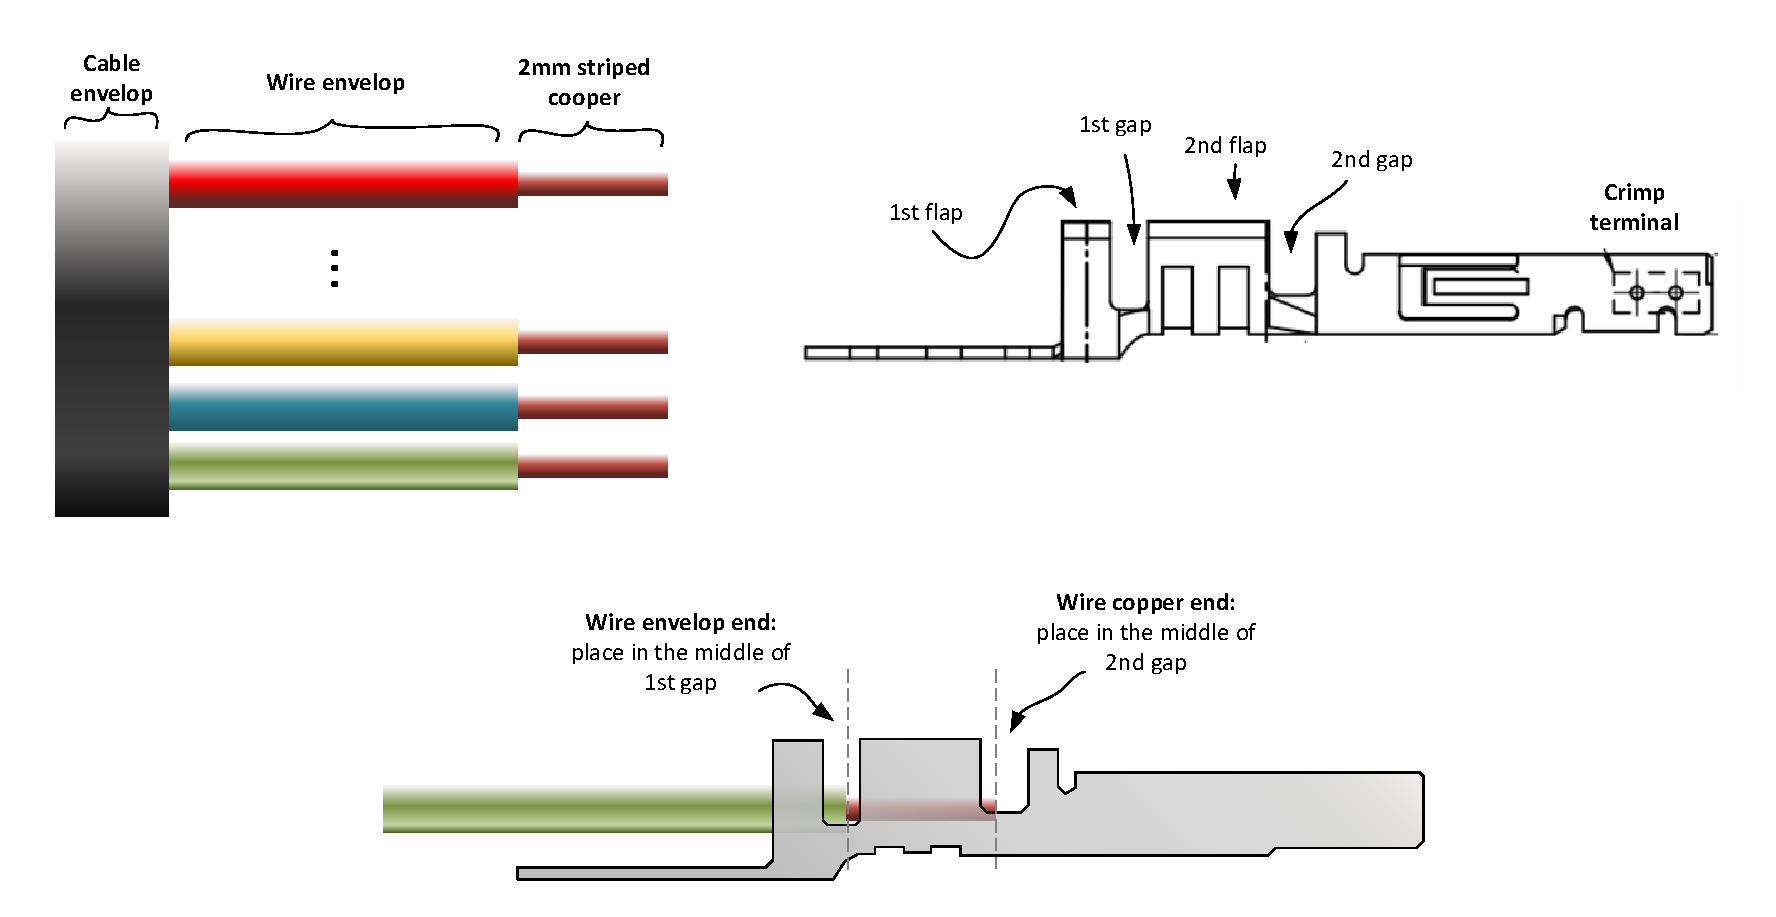
\includegraphics[angle=90,width=1\columnwidth]{figs/body03/FIGCRIMPmicro1.pdf}\\
  \caption[Crimping Molex Micro-Fit 3.0\texttrademark: placing the crimp terminal]{Crimping Molex Micro-Fit 3.0\texttrademark: placing the crimp terminal}
  \label{FIG:CRIMPmicro1}
\end{figure}
\begin{figure}
  \centering
  % Requires \usepackage{graphicx}
  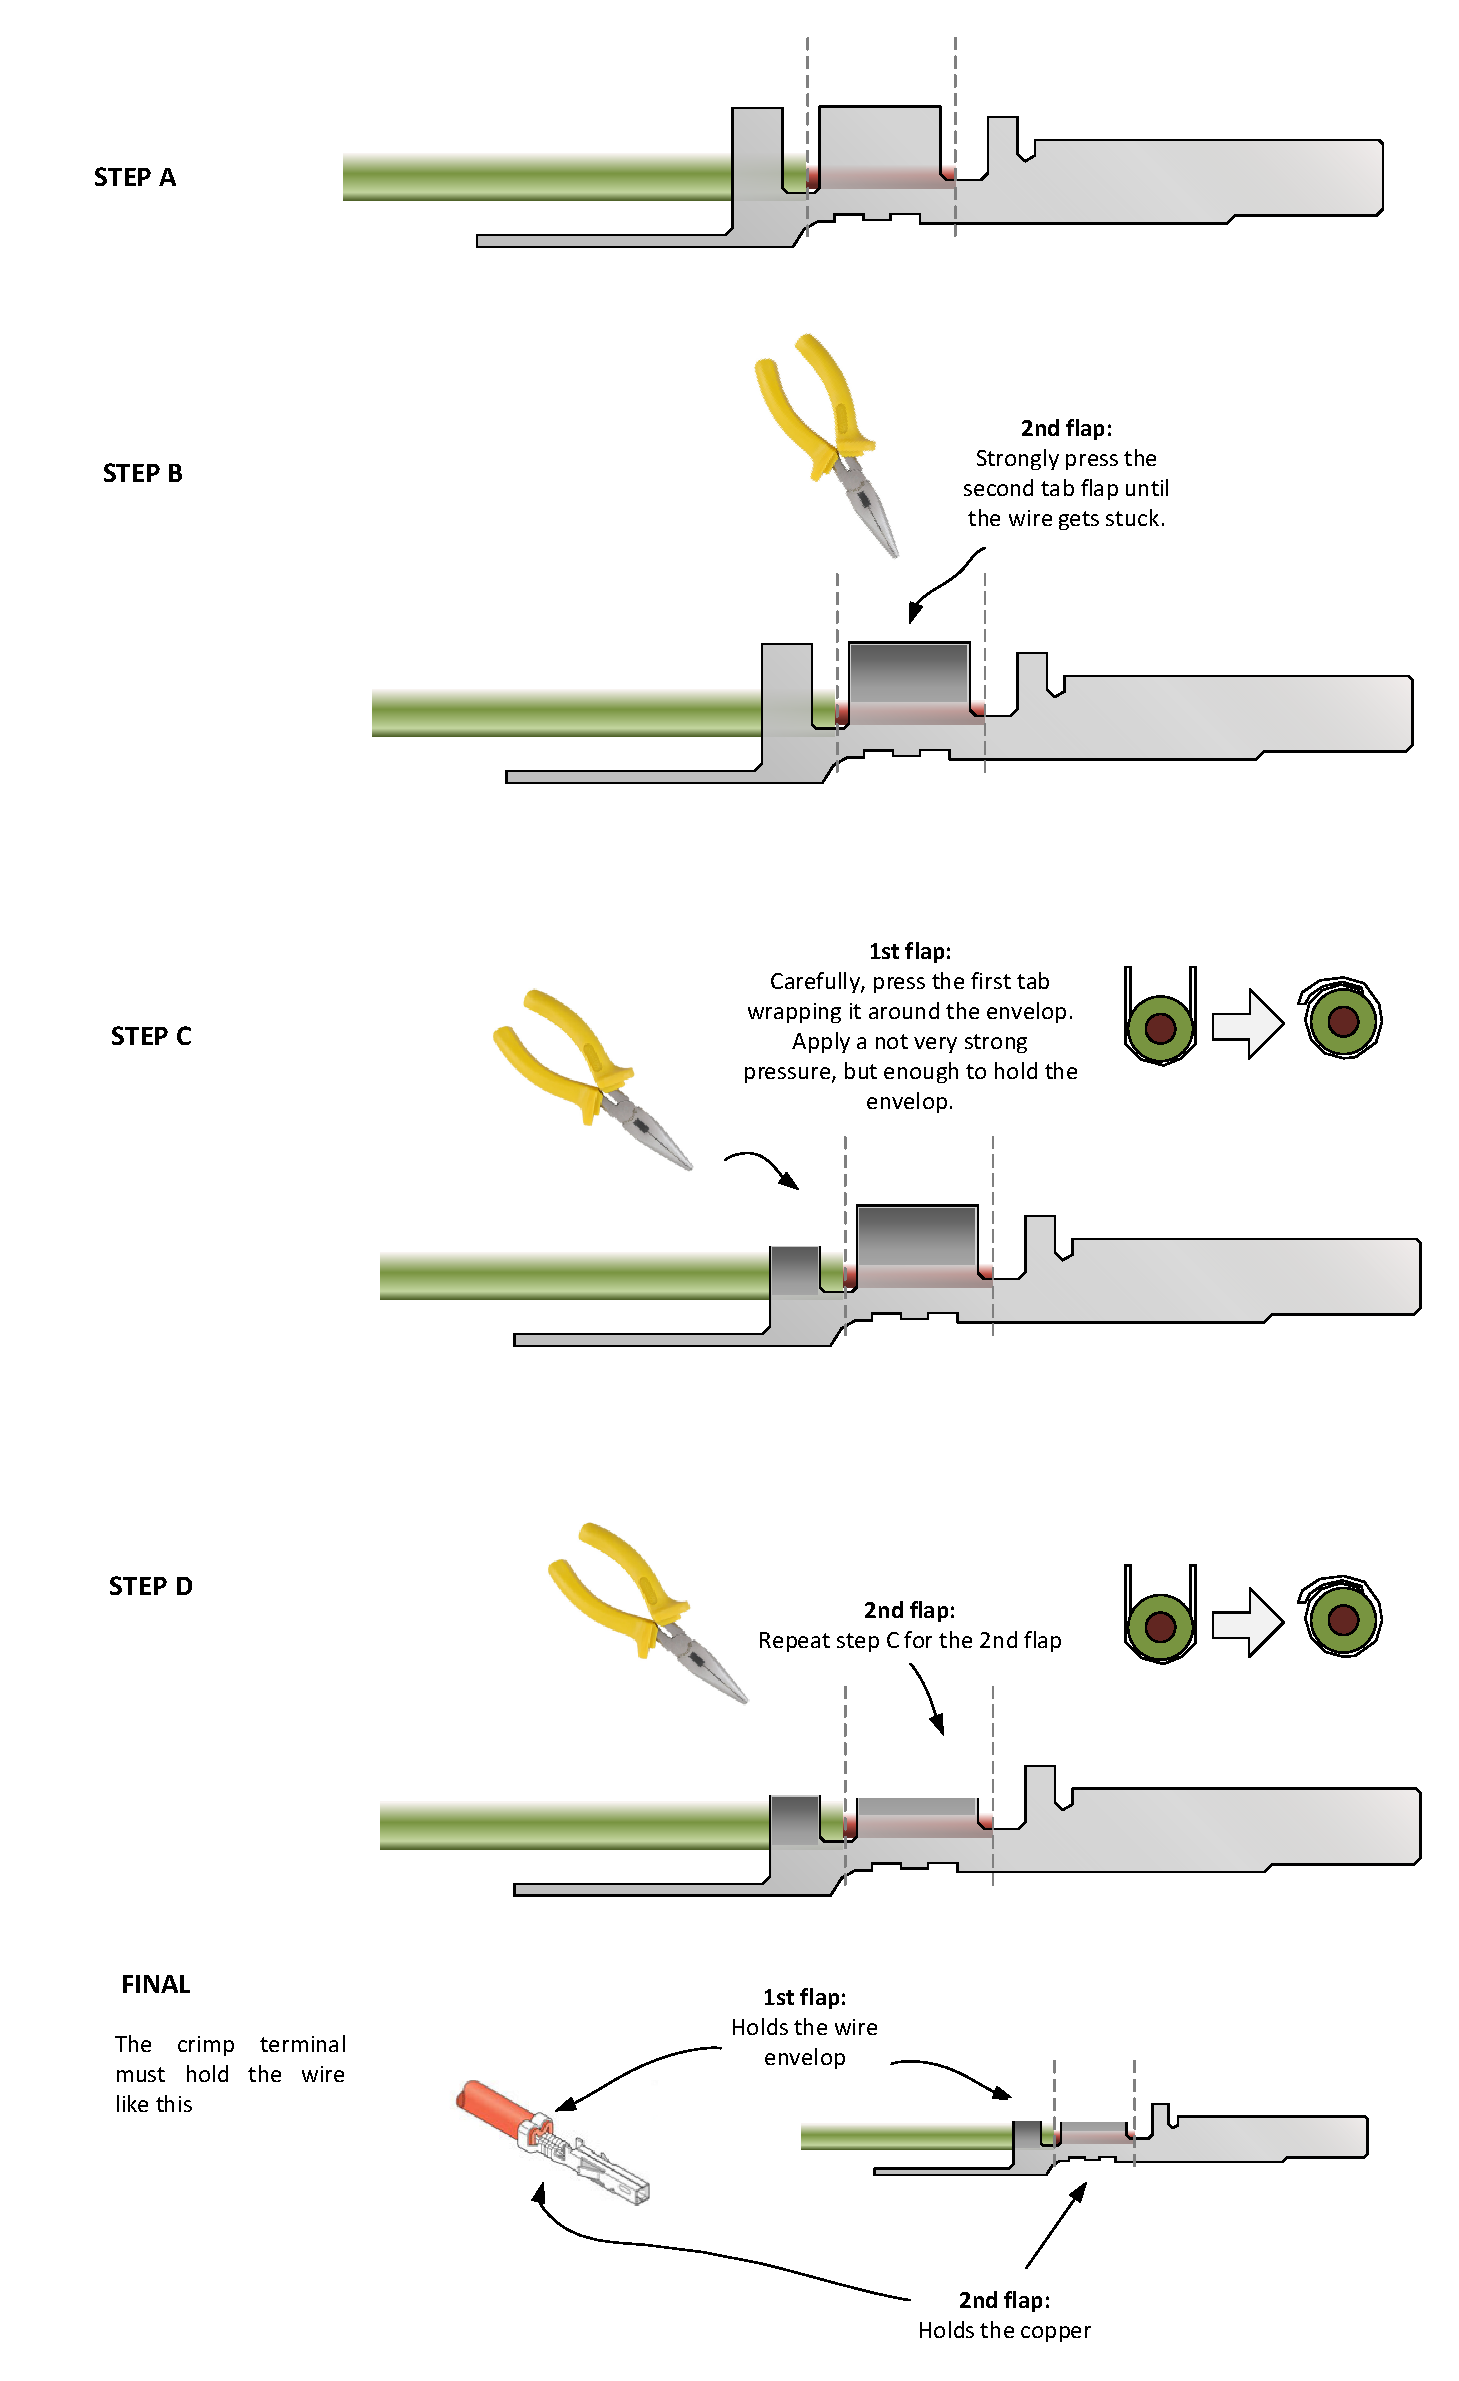
\includegraphics[angle=90,width=1\columnwidth]{figs/body03/FIGCRIMP2.pdf}\\
  \caption[Crimping Molex Micro-Fit 3.0\texttrademark: procedures for manual crimping]{Crimping Molex Micro-Fit 3.0\texttrademark: procedures for manual crimping}
  \label{FIG:CRIMP2}
\end{figure}
\begin{figure}
  \centering
  % Requires \usepackage{graphicx}
  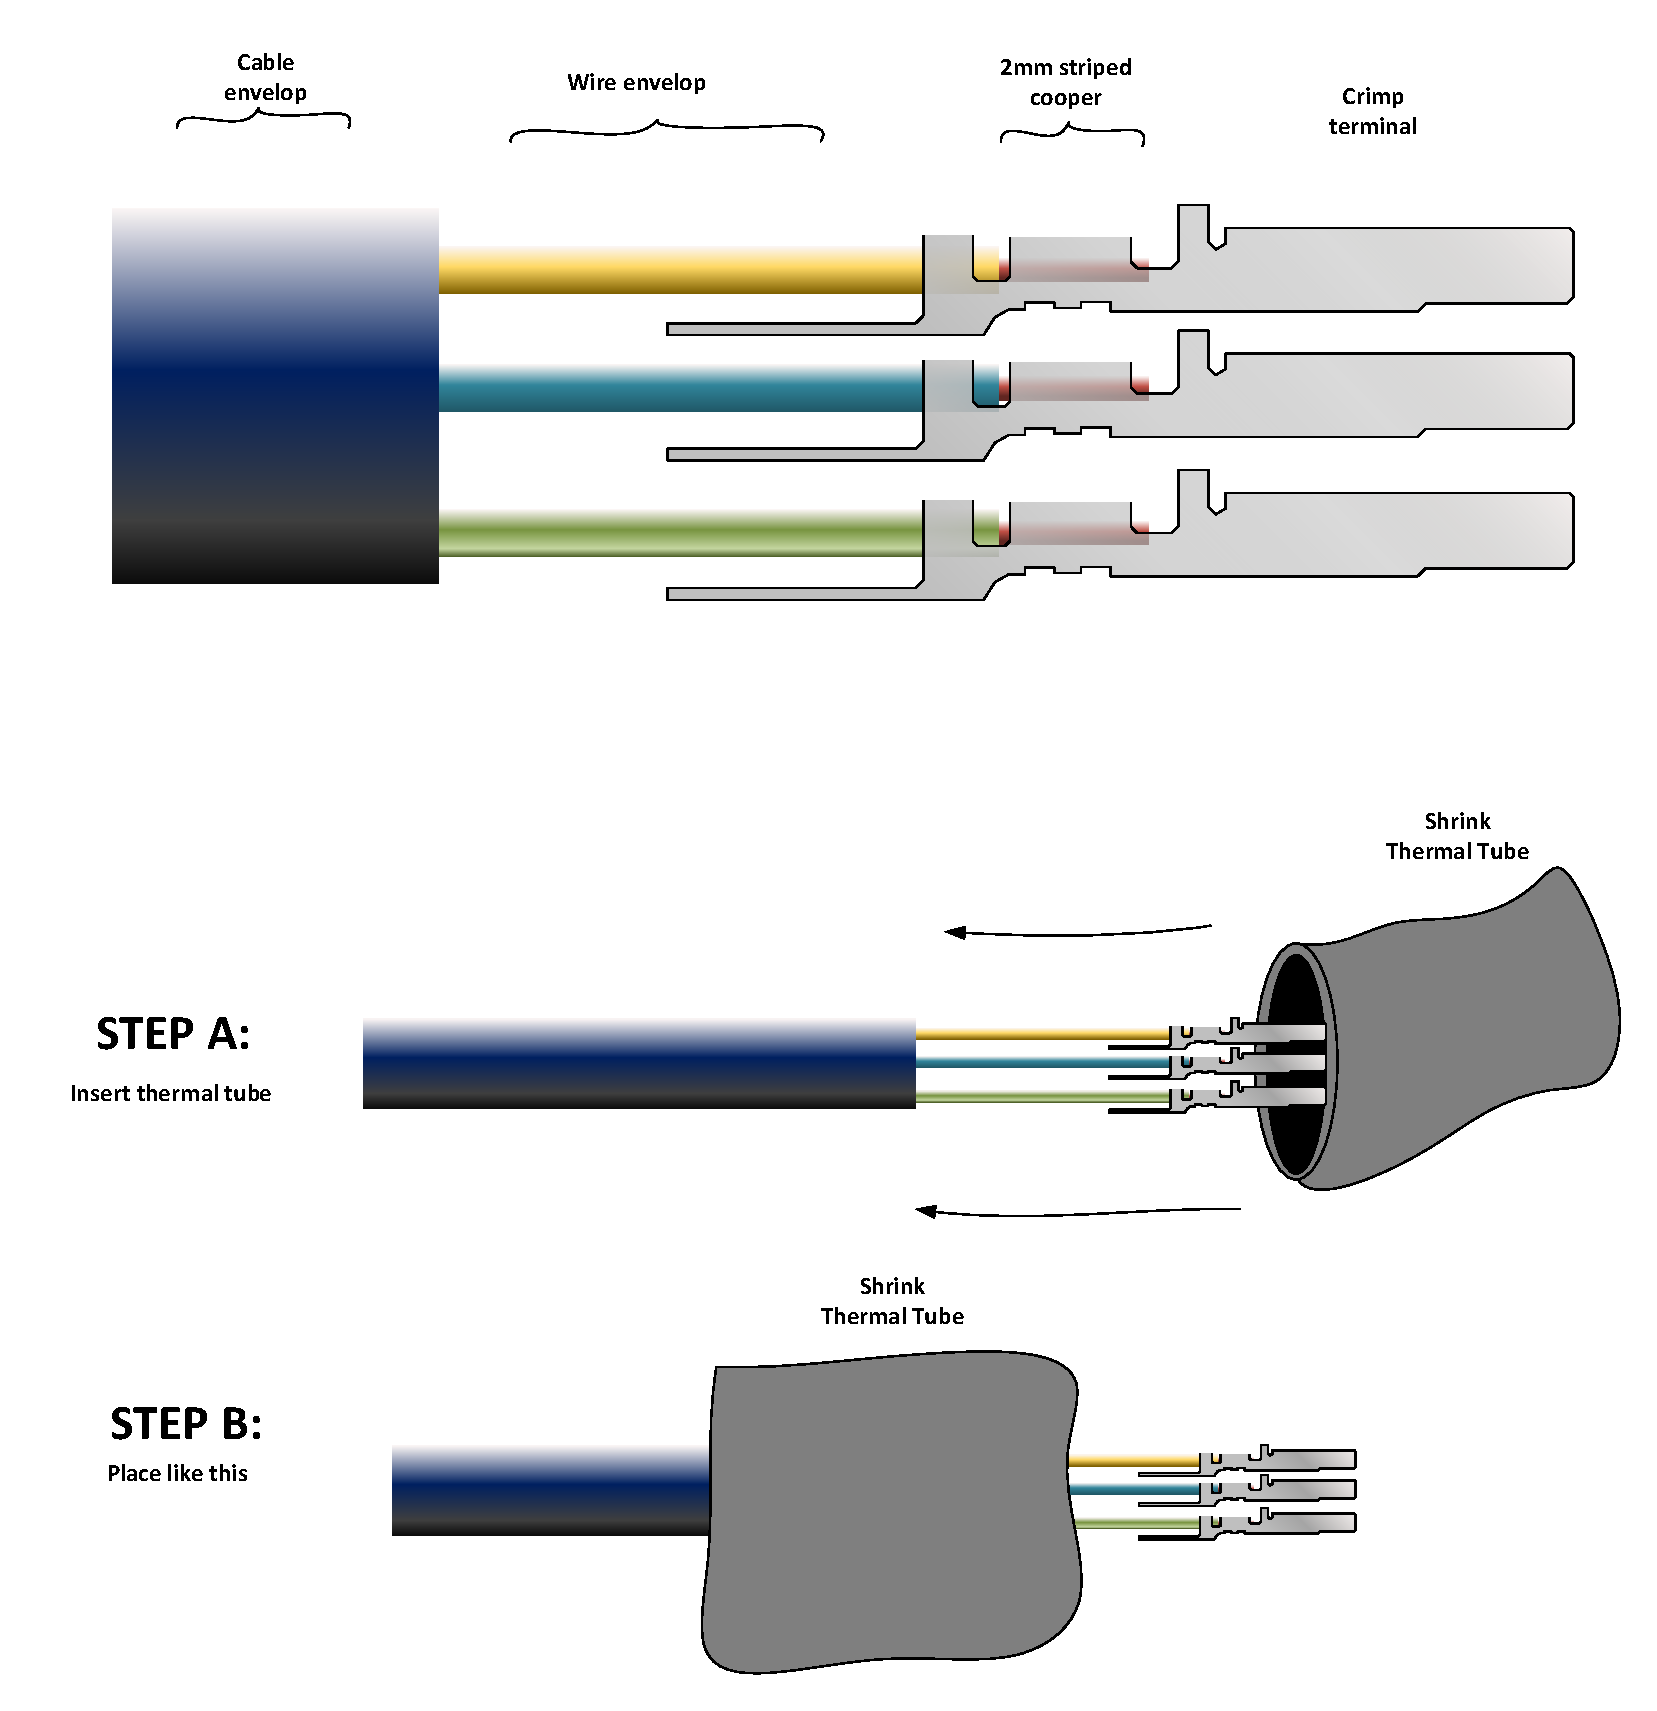
\includegraphics[angle=90,width=1\columnwidth]{figs/body03/FIGCRIMP3.pdf}\\
  \caption[Crimping Molex Micro-Fit 3.0\texttrademark: applying the heat shrink tube]{Crimping Molex Micro-Fit 3.0\texttrademark: applying the heat shrink tube}
  \label{FIG:CRIMP3}
\end{figure}
\begin{figure}
  \centering
  % Requires \usepackage{graphicx}
  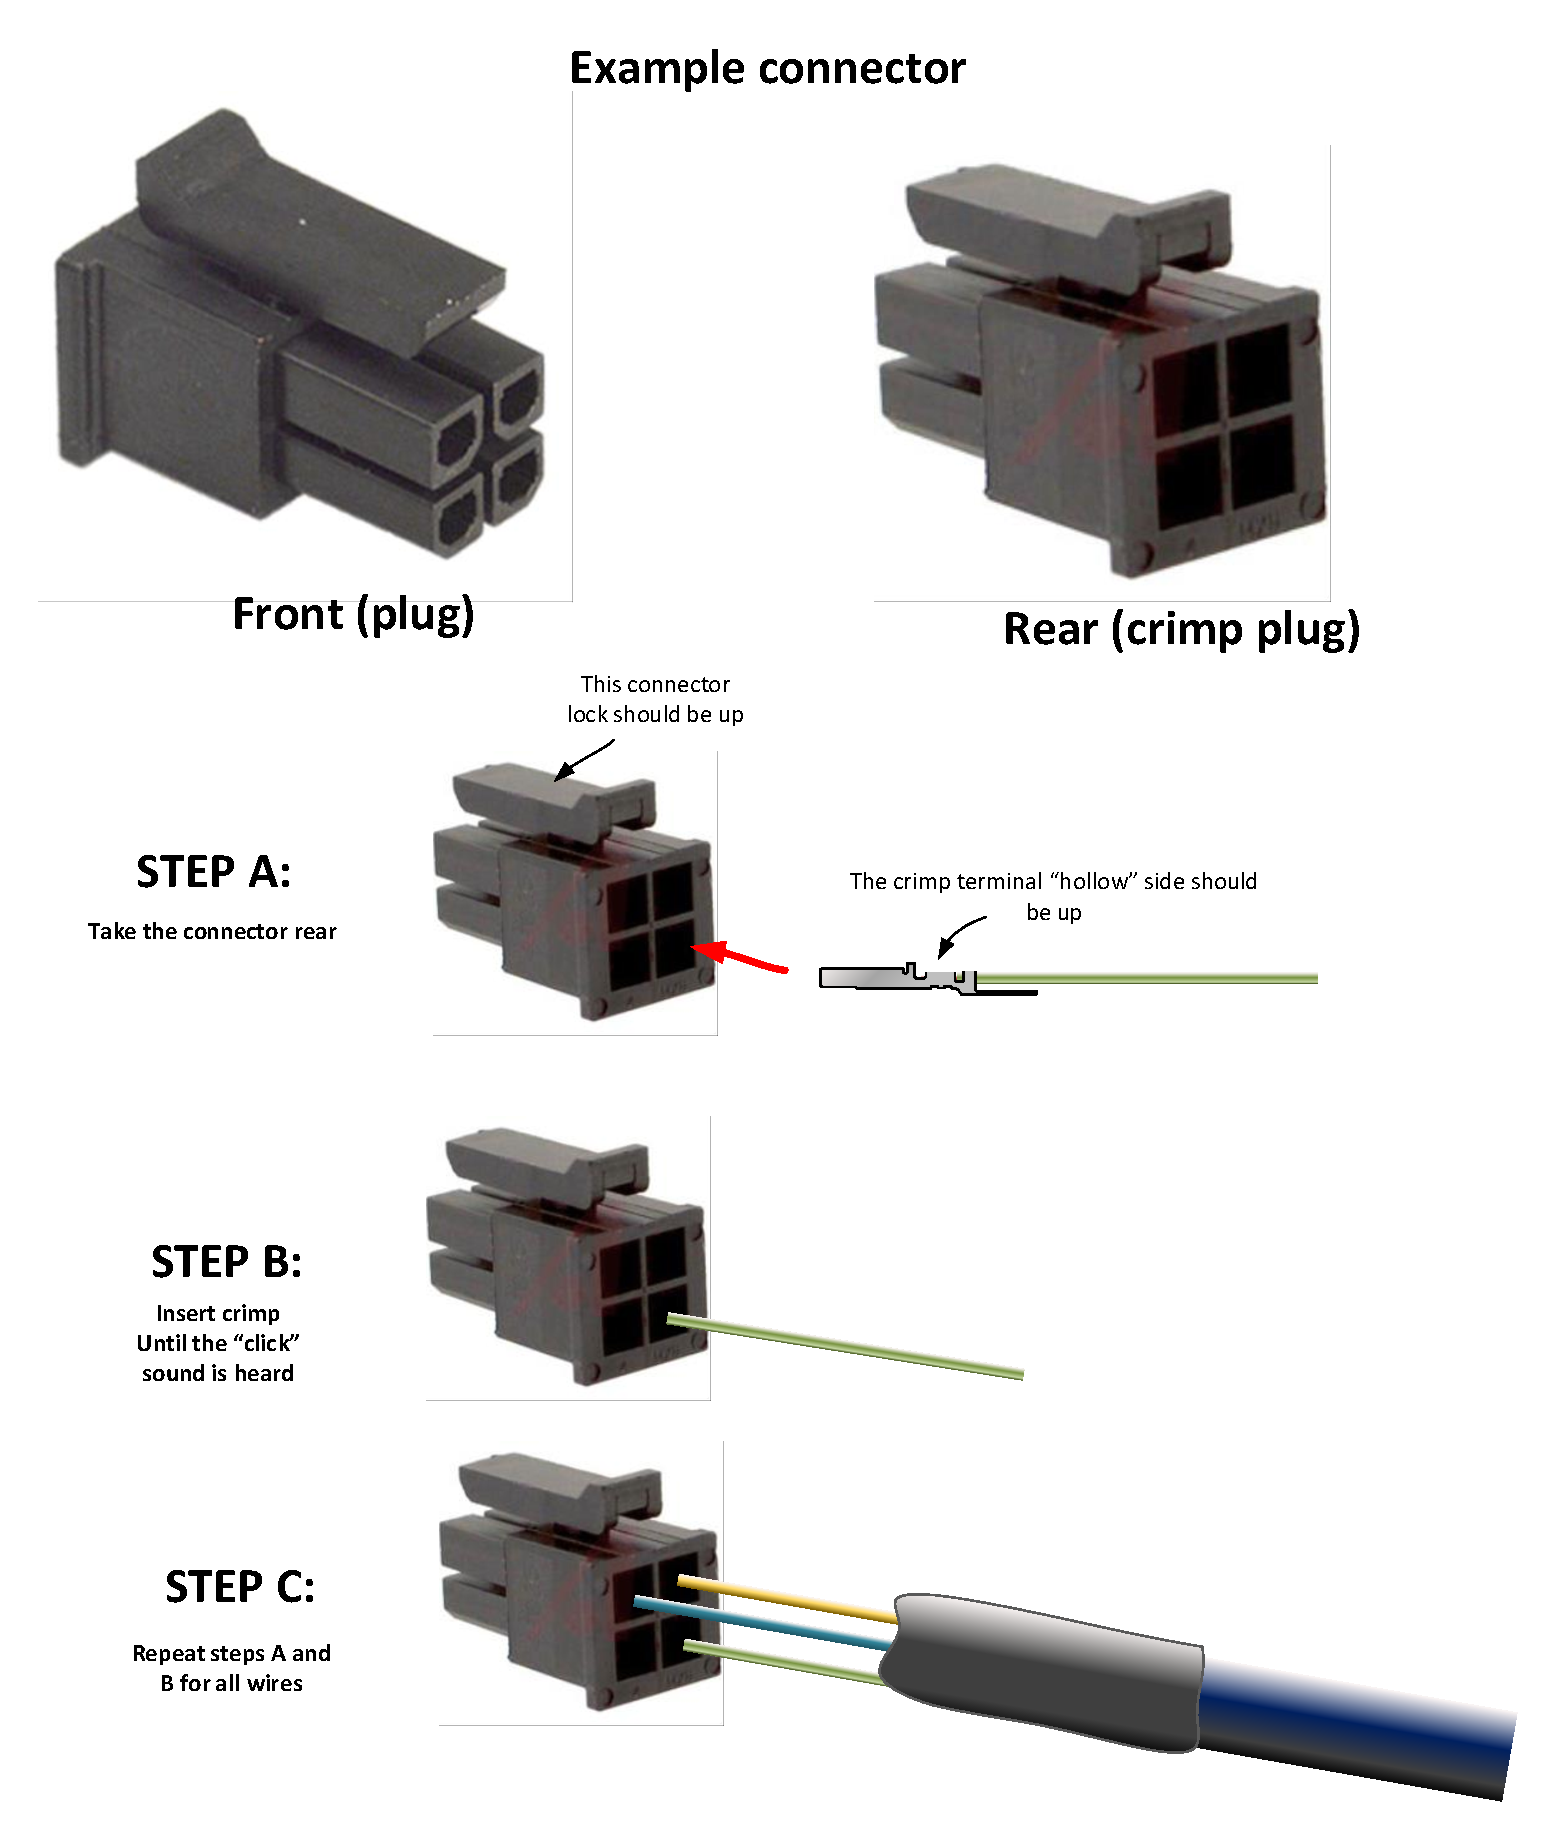
\includegraphics[angle=90,width=1\columnwidth]{figs/body03/FIGCRIMP4.pdf}\\
  \caption[Crimping Molex Micro-Fit 3.0\texttrademark: inserting the crimp terminals into the connector holes]{Crimping Molex Micro-Fit 3.0\texttrademark: inserting the crimp terminals into the connector holes}
  \label{FIG:CRIMP4}
\end{figure}
\subsubsection{Crimping Molex Mini-Fit\textregistered Family} \label{CRIMPINGmini}
For connecting wires to a Molex Mini-Fit\textregistered connector from 39-01-xxxx family (sections~\ref{DEVICE:miniMotor} and~\ref{DEVICE:miniPower}), you first need to crimp the edge of these wires in the Molex crimp terminal from 44476-xxxx family (section~\ref{DEVICE:miniCrimp}). For this, you should perform the following steps:
\begin{enumerate}
  \item Use the tool "Molex Hand Crimper Tool Part Number: 63819-0900" (see section~\ref{DEVICE:TOOLCRIMPERmini}).
  \item For each wire to be connected, use a cutting plier (like the one described in section~\ref{DEVICE:TOOLPLIERCUTTING}), strip the wire envelop, leaving 3mm copper exposed.
  \item Place the wire and the crimp terminal according to figure~\ref{FIG:CRIMPmini5}.
  \item Use the Molex Hand Crimper (item 1) to crimp the wire.
  \item If the crimping tool is not available, perform these steps:
  \begin{itemize}
    \item Using a preheated soldering station (like the one presented in section~\ref{DEVICE:TOOLSOLDERINGSTATION}), tin the 3mm striped copper wire.
    \item Place the wire/crimp terminal like described in item 3.
    \item Use a long needle-nose plier (like the one presented in section~\ref{DEVICE:TOOLPLIERNEEDLENOSE}) to press the crimp flaps, following the steps described in figure~\ref{FIG:CRIMP6}.
    \item Using the preheated soldering station, touch the iron tip over the crimp terminal for long enough until the internal welding tin (on the wire tip surface) gets melted.
  \end{itemize}
  \item Repeat the previous steps for each wire.
  \item Envelop the whole wire set using 2cm of a heat shrink tube (like the ones described in section~\ref{DEVICE:TOOLTHERMALINSULATION}). Select the correct tube diameter according to your need. Use figure~\ref{FIG:CRIMP7} as a reference.
  \item Use the heat of a thermal blower (like the one described in section~\ref{DEVICE:TOOLTHERMALBLOWER}) to shrink the thermal tube around the cable/wires.
  \item Using the correct pinout for the concerning connector (which can be checked in section~\ref{DEVICE:CONNECTORS}), insert each crimped terminal into the respective connector hole. A "click" sound must be heard, and this indicates that the crimp terminal is in the correct position and cannot be removed. Use figure~\ref{FIG:CRIMP8} as a reference.
\end{enumerate}
\begin{figure}
  \centering
  % Requires \usepackage{graphicx}
  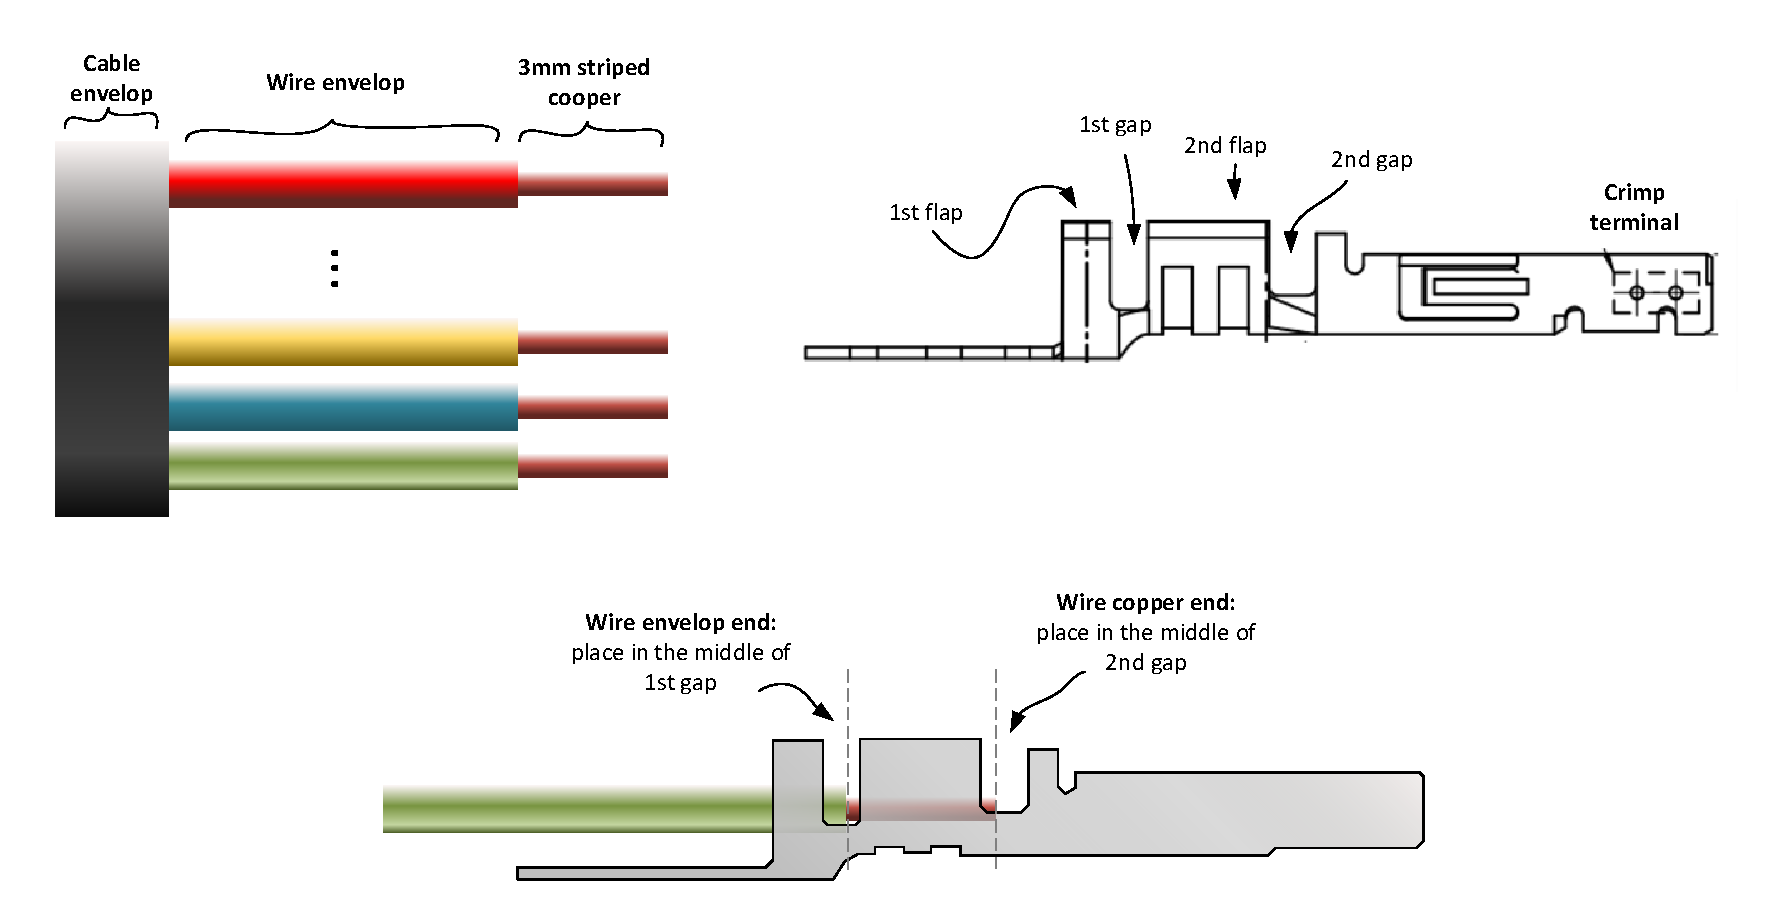
\includegraphics[angle=90,width=1\columnwidth]{figs/body03/FIGCRIMPmini5.pdf}\\
  \caption[Crimping Molex Mini-Fit \textregistered: placing the crimp terminal]{Crimping Molex Mini-Fit \textregistered: placing the crimp terminal}
  \label{FIG:CRIMPmicro5}
\end{figure}
\begin{figure}
  \centering
  % Requires \usepackage{graphicx}
  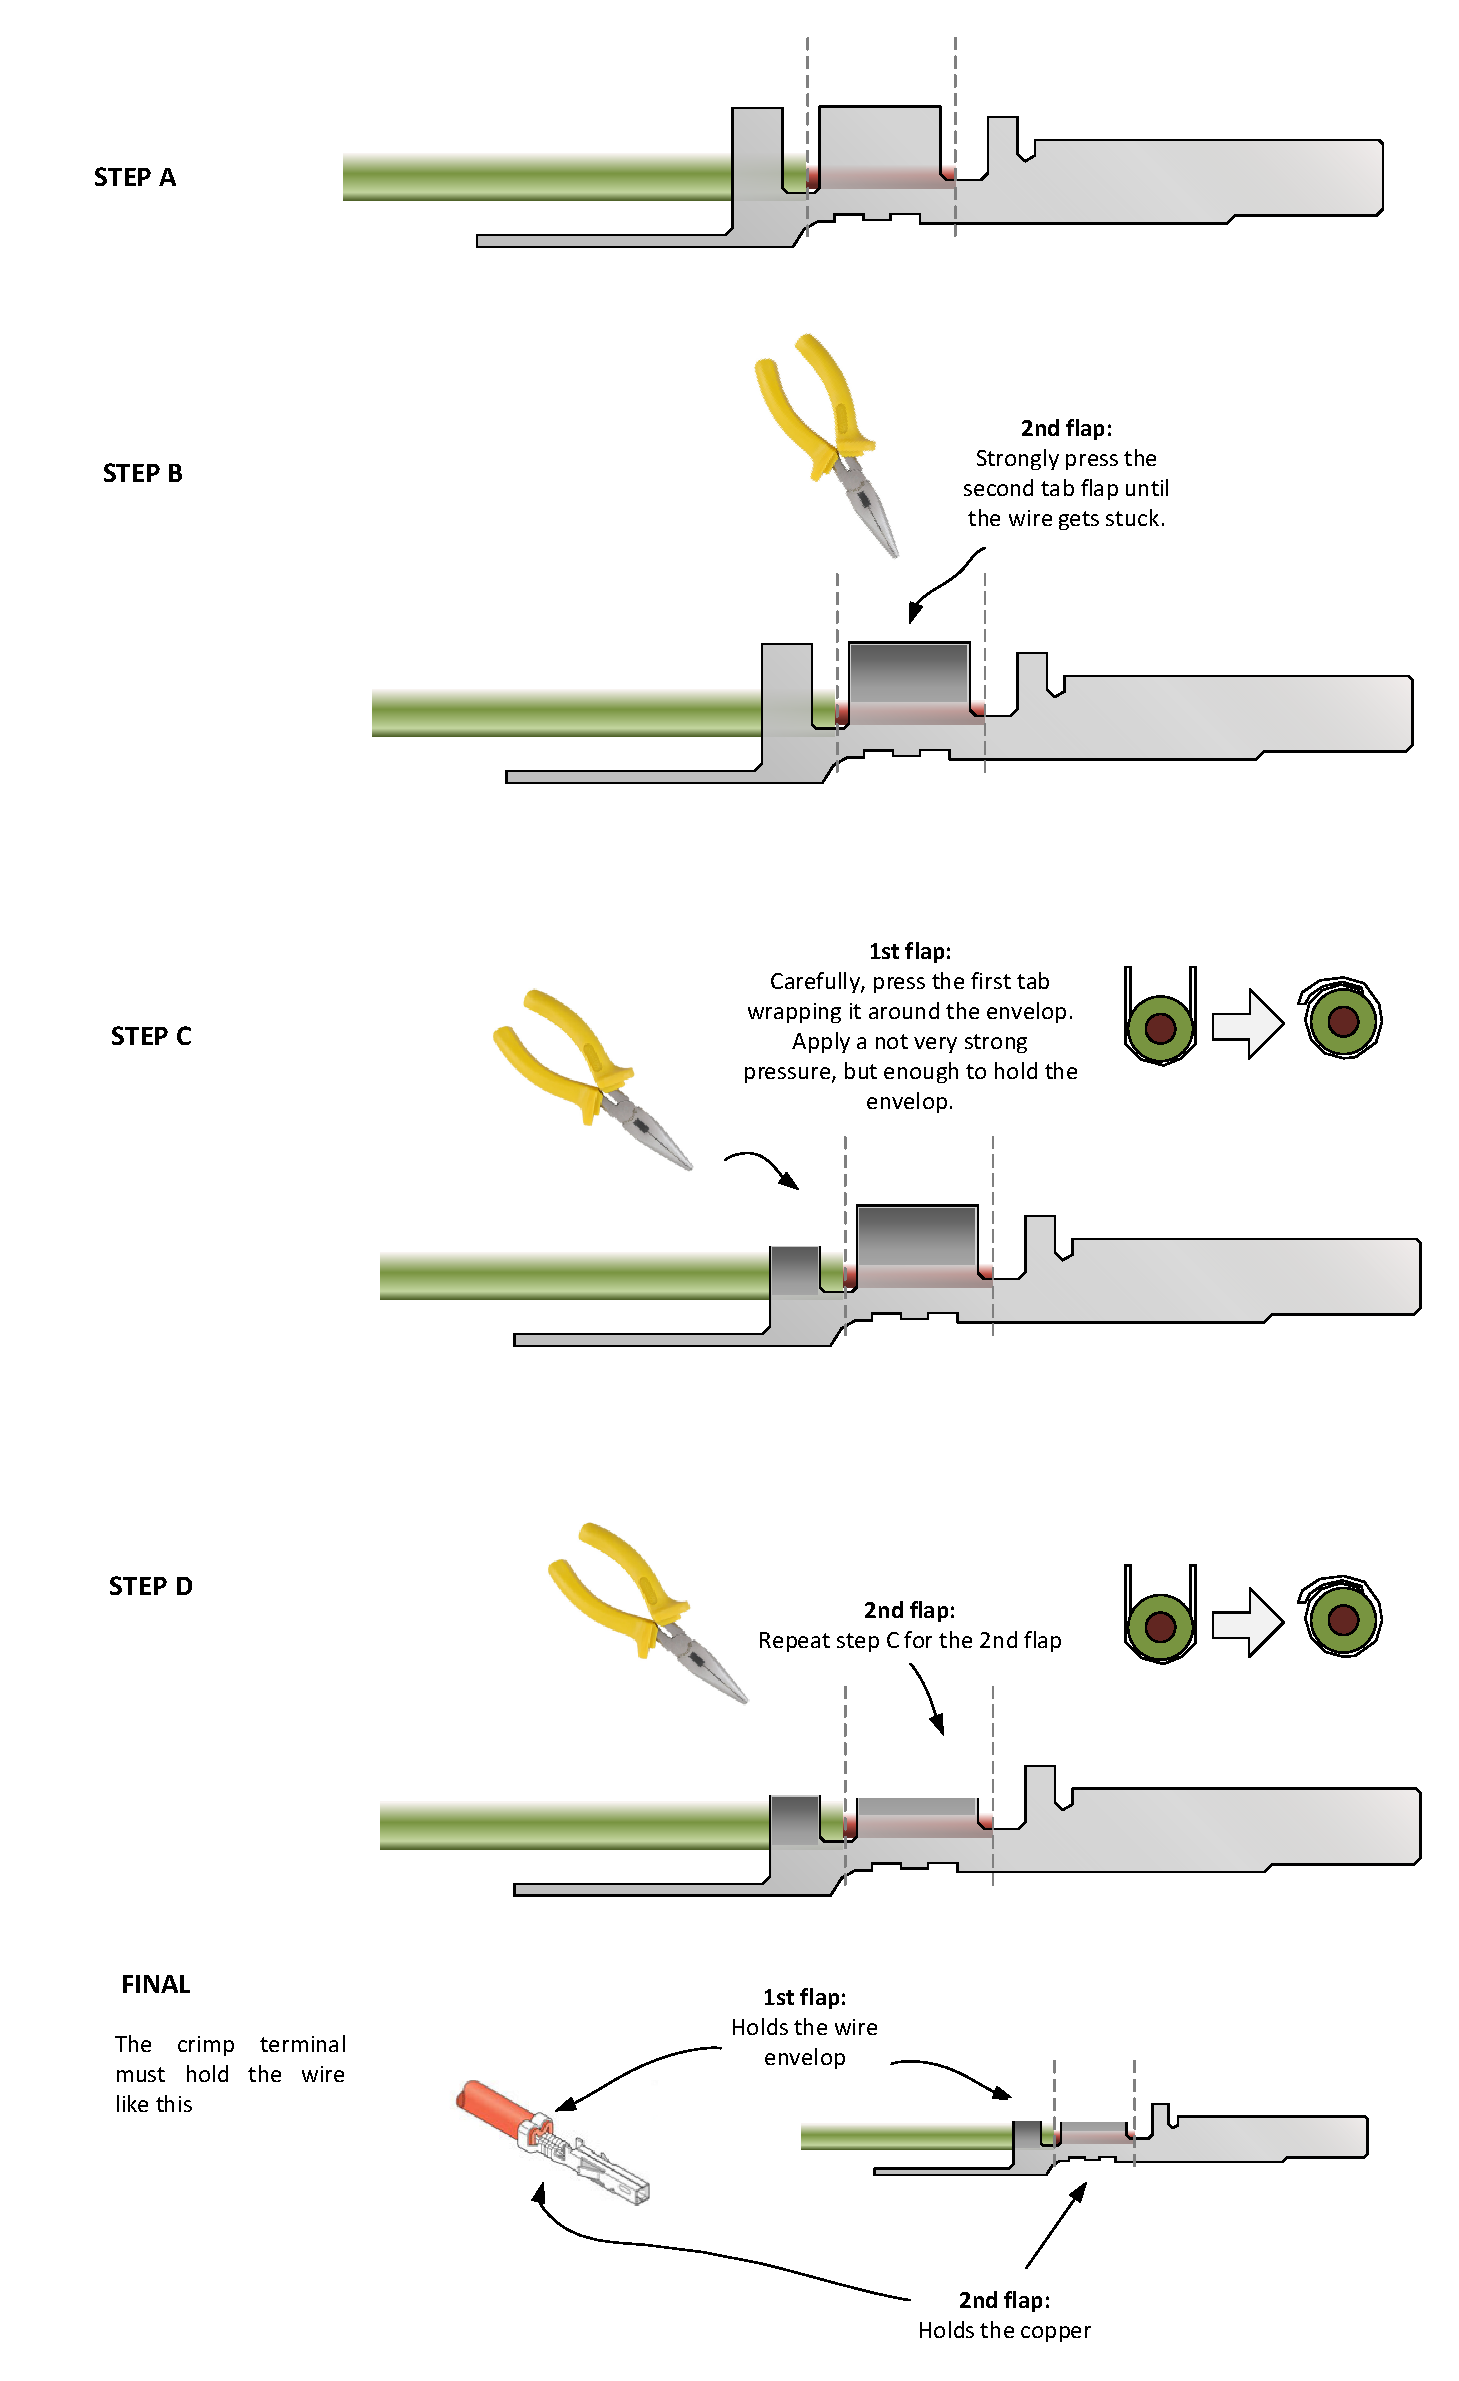
\includegraphics[angle=90,width=1\columnwidth]{figs/body03/FIGCRIMP6.pdf}\\
  \caption[Crimping Molex Mini-Fit \textregistered: procedures for manual crimping]{Crimping Molex Mini-Fit \textregistered: procedures for manual crimping}
  \label{FIG:CRIMP6}
\end{figure}
\begin{figure}
  \centering
  % Requires \usepackage{graphicx}
  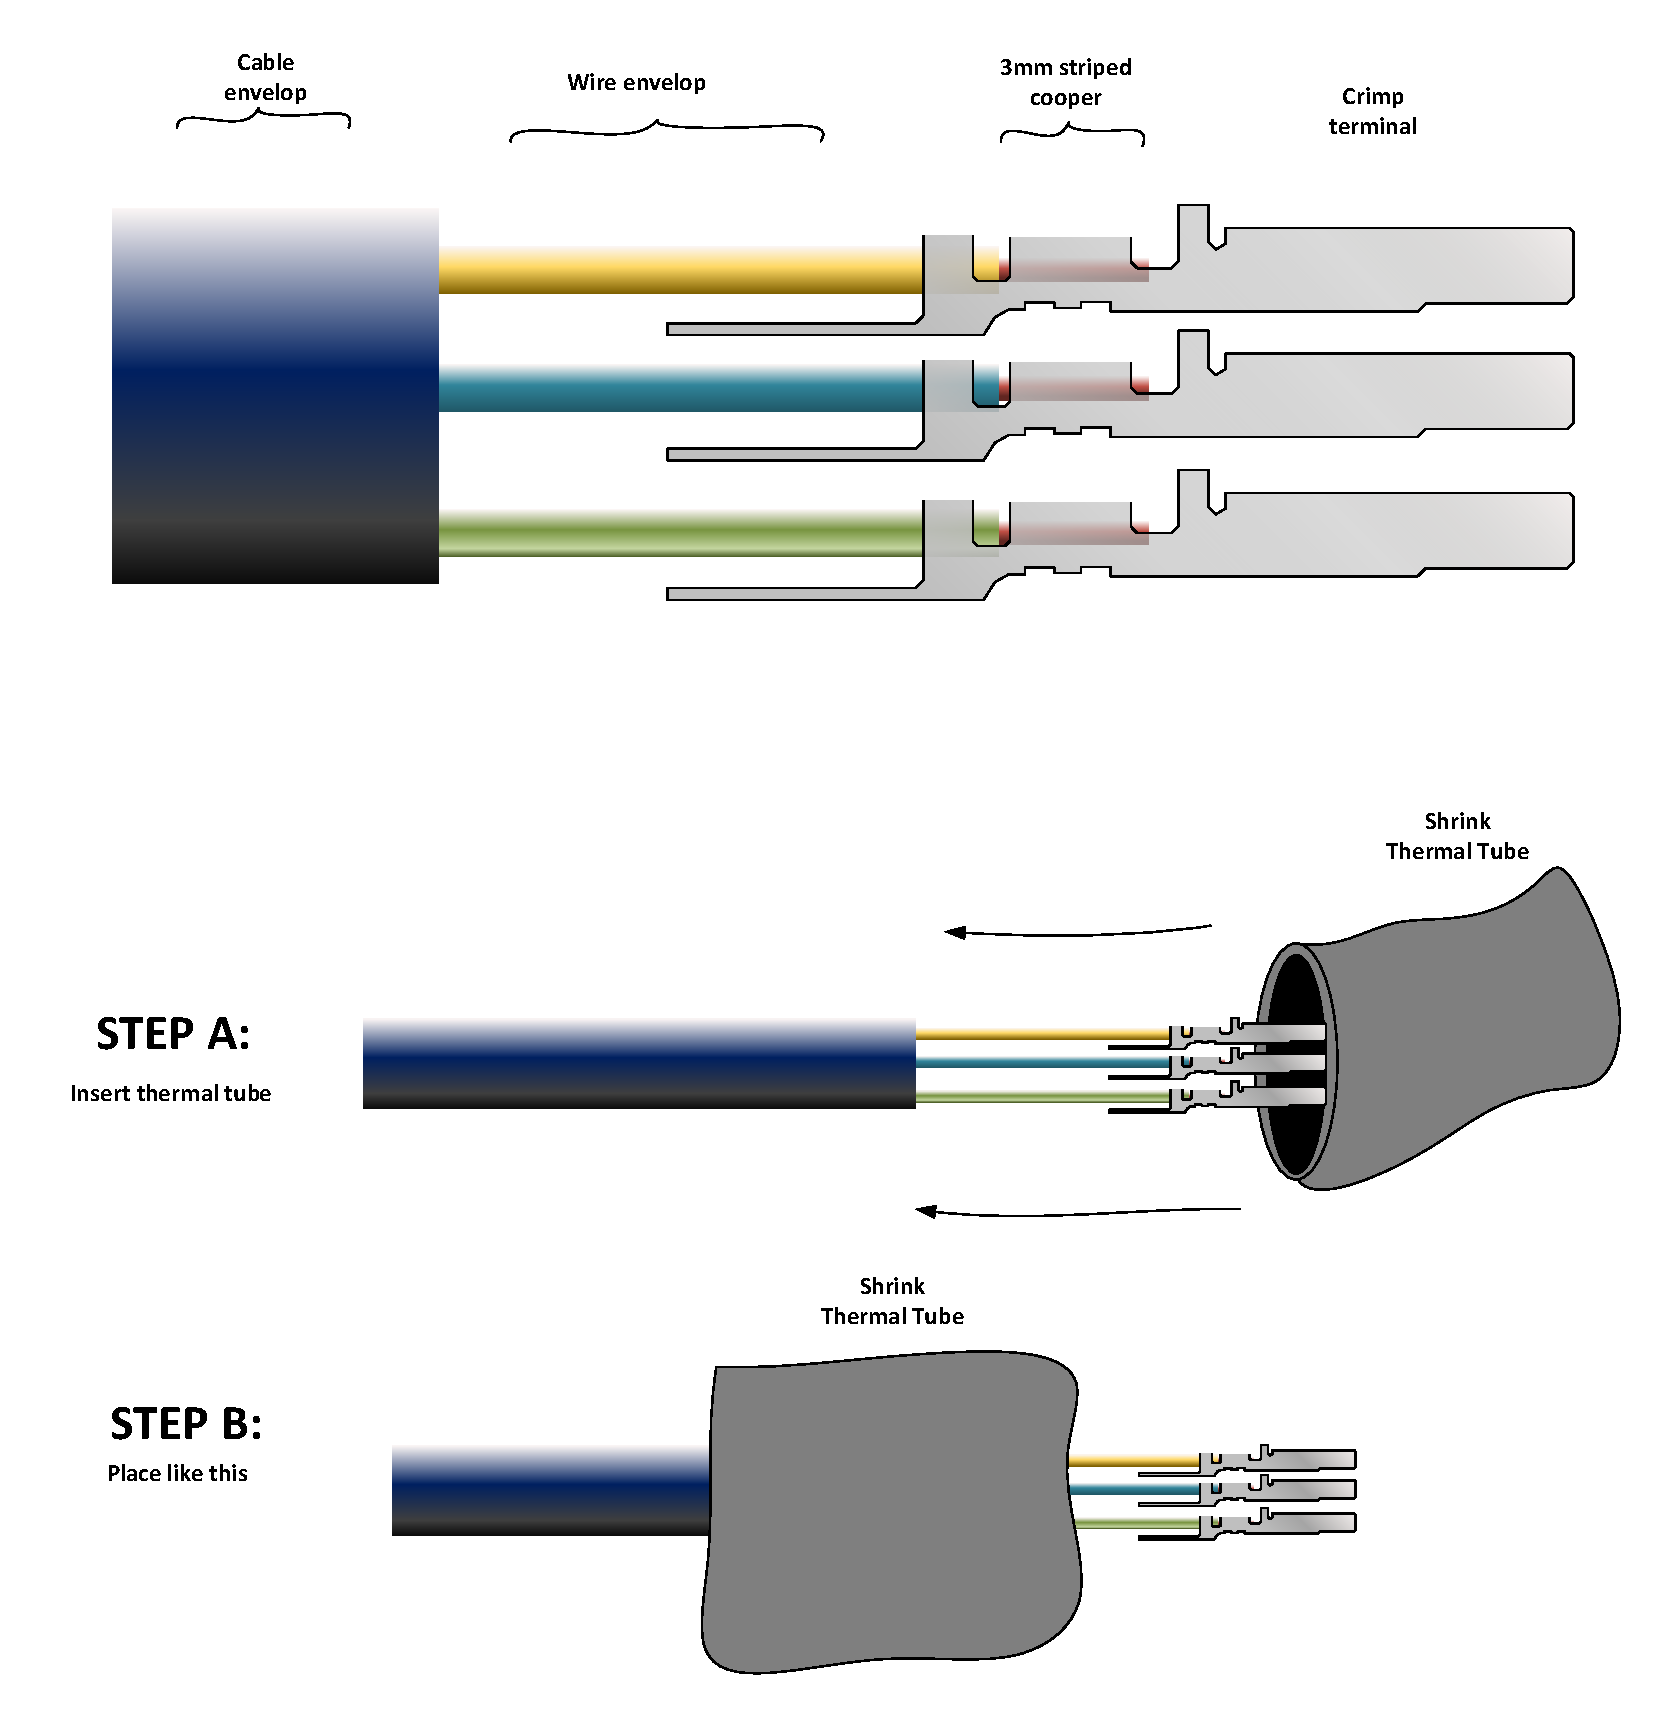
\includegraphics[angle=90,width=1\columnwidth]{figs/body03/FIGCRIMP7.pdf}\\
  \caption[Crimping Molex Mini-Fit \textregistered: applying the heat shrink tube]{Crimping Molex Mini-Fit \textregistered: applying the heat shrink tube}
  \label{FIG:CRIMP7}
\end{figure}
\begin{figure}
  \centering
  % Requires \usepackage{graphicx}
  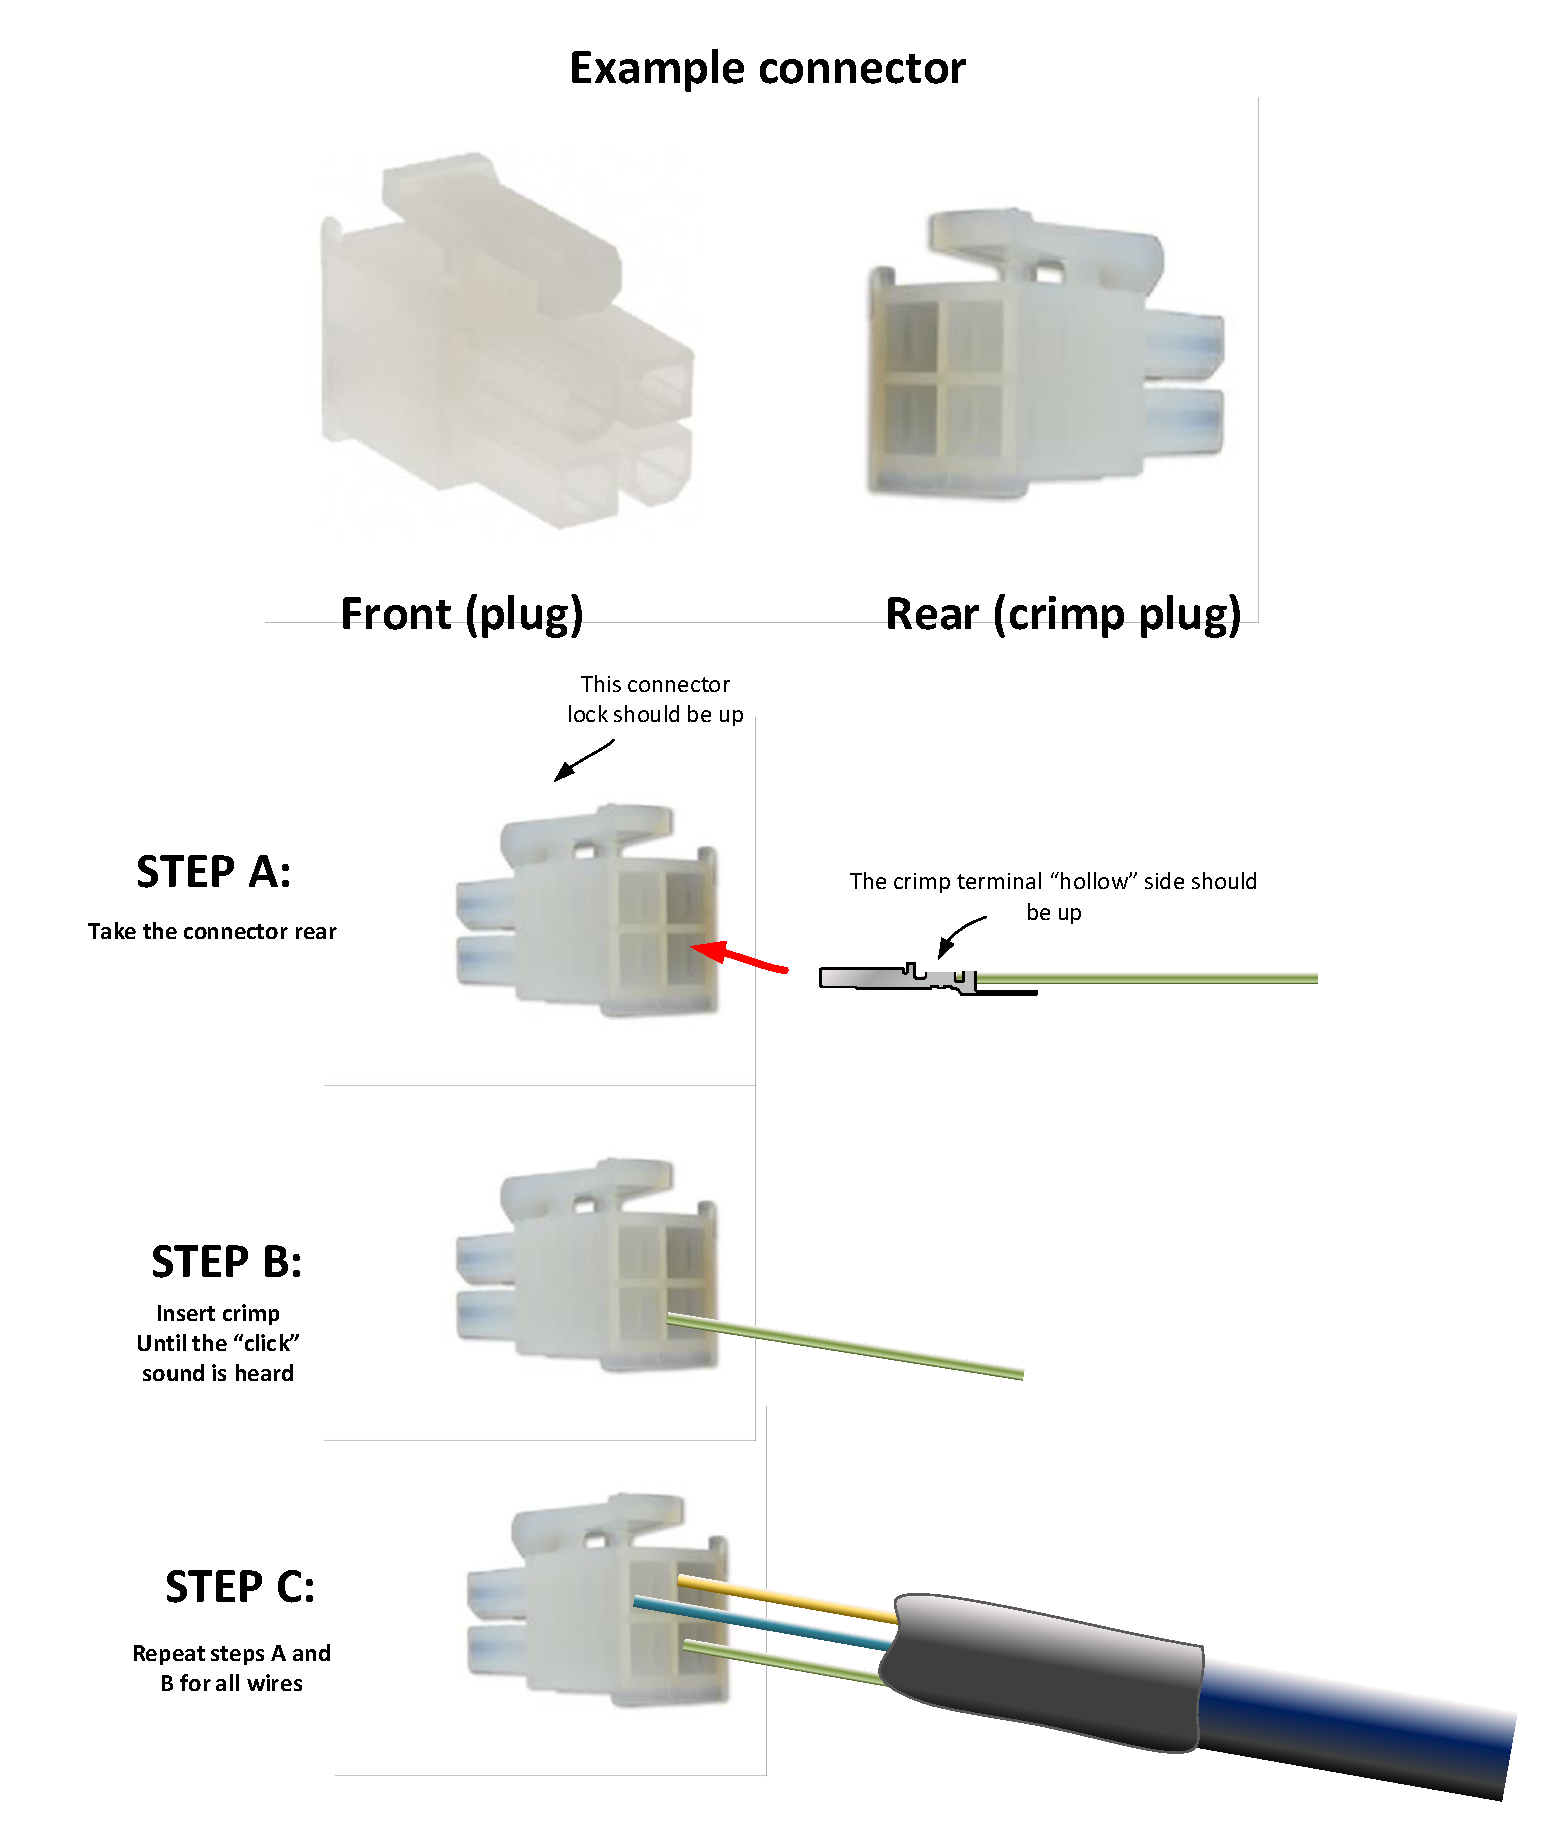
\includegraphics[angle=90,width=1\columnwidth]{figs/body03/FIGCRIMP8.pdf}\\
  \caption[Crimping Molex Mini-Fit \textregistered: inserting the crimp terminals into the connector holes]{Crimping Molex Mini-Fit \textregistered: inserting the crimp terminals into the connector holes}
  \label{FIG:CRIMP8}
\end{figure}
\subsection{Printed circuit boards (PCB) fabrication and assembly}
\section{System installation on site}
\section{System testing on site}
\section{System commissioning} 